\section{Experiments}
\label{sec:results}

We generate 16 attempts for each of 1,000 questions (dev 200, test 400, extra 400) with the mixed adapter, and judge
every answered attempt with the same adapter. All settings are tuned on dev and evaluated on test $\cup$ extra.

\paragraph{The pipeline reproduces Phase 2, and the model predicts the scaling curves.}
The Phase-3 pools match the Phase-2 numbers:
\begin{itemize}
\item \textbf{Dev:} single attempt $69.8\%$, pass@4 $86.3\%$, majority@4 $78.1\%$ (Phase~2: $69.8$, $86.5$, $77.5$).
\item \textbf{Test:} $67.0$, $82.8$, $74.9$ (Phase~2: $67.4$, $82.8$, $74.0$).
\end{itemize}
The model was fitted only to the Phase-2 4-attempt aggregates. On test it predicts majority@8 $=77.5$ (observed
$77.5$), majority@16 $=78.2$ (observed $78.7$) and pass@16 $=90.8$ (observed $90.2$). It also predicts the share of
4-attempt configurations where the majority is already right ($71.7\%$ vs $72.3\%$) and where no attempt is right
($17.2\%$ vs $17.3\%$).

Majority vote saturates at the predicted limit ($78.3\%$) while pass@16 reaches $90.2\%$ (Figure~\ref{fig:scaling}).
On test, adaptive-consistency reaches the same plateau ($78.7\%$) with fewer attempts but cannot pass it.

\paragraph{Judge-free features already reach the trained judge's pooled AUROC.}
Table~\ref{tab:trace} scores attempts by length, by counts of self-correction phrases, or by guess phrases.

\begin{itemize}
\item \textbf{Pooled:} these features reach AUROC 0.65--0.70, the level the Phase-2 trained self-judge reached
  (0.665). Hard questions produce long, hesitant attempts.
\item \textbf{Within question:} 0.54--0.61.
\item \textbf{Contested questions:} 0.46--0.58, about chance. This is where picking happens (\S\ref{sec:headroom}).
\end{itemize}

The table is the invariance theorem in miniature: a large pooled AUROC that selection cannot use.

The same data support the liveness account (Appendix~\ref{app:proofs}): $98$--$99\%$ of \emph{right} attempts contain
self-corrections, about 25 per attempt (36 per wrong attempt). A detector of ``an error occurred somewhere'' therefore
fires on almost every trace. What decides correctness is whether an error is still live at the end.

\begin{table*}[t]
\centering\small
\resizebox{\linewidth}{!}{\begin{tabular}{@{}llcccc@{}}
\toprule
Set & Trace feature & Pooled AUROC & Within-question & Contested within & Mean (right / wrong) \\
\midrule
dev & Length (tokens) & 0.700 & 0.580 & 0.495 & 7521.8 / 10005.3 \\
dev & Self-corrections (``wait'', ``actually'', \dots) & 0.677 & 0.563 & 0.477 & 23.8 / 34.9 \\
dev & Guess phrases (``let's assume'', \dots) & 0.680 & 0.611 & 0.577 & 1.0 / 2.4 \\
dev & Final-answer tags & 0.529 & 0.549 & 0.488 & 1.0 / 1.2 \\
test & Length (tokens) & 0.655 & 0.573 & 0.486 & 7977.9 / 9750.5 \\
test & Self-corrections (``wait'', ``actually'', \dots) & 0.648 & 0.553 & 0.514 & 26.0 / 36.0 \\
test & Guess phrases (``let's assume'', \dots) & 0.656 & 0.576 & 0.568 & 1.1 / 2.3 \\
test & Final-answer tags & 0.526 & 0.536 & 0.509 & 1.0 / 1.1 \\
\bottomrule
\end{tabular}}
\caption{Judge-free trace features. They reach the pooled AUROC of the Phase-2 trained self-judge (0.665) because hard questions produce long, hesitant attempts, but are near chance on contested questions, where picking happens. Almost every right attempt contains self-corrections.}
\label{tab:trace}
\end{table*}


\subsection{Stage 0: what the judge knows}
\label{sec:stage0}

Table~\ref{tab:stage0} tests the leniency account of \S\ref{sec:lenient} on test attempts 0--3, judged with four
chains each.

\begin{itemize}
\item \textbf{The judge is lenient.} It says ``incorrect'' to about one attempt in seven; $d'=0.49$.
\item \textbf{Sampled verdicts look near chance.} One verdict gives AUROC $0.57$; the share of four gives $0.64$.
\item \textbf{Probabilities recover the signal.} The verdict probability averaged over the four chains, and the
  direct probability read with no reasoning at all, reach $0.69$--$0.71$. That is the latent AUROC the model
  inferred from Phase-2 flag rates alone ($0.715$). Both paired differences from the four-verdict share are
  significant: $+0.067$ $[+0.047, +0.085]$ and $+0.090$ $[+0.049, +0.130]$ (paired bootstrap over questions).
\item \textbf{Verdicts on one attempt are strongly correlated.} Four ``incorrect'' verdicts on the same wrong attempt
  occur about $12\times$ as often as independent verdicts would allow. This is the persistent per-attempt component
  of Eq.~\ref{eq:judge}.
\end{itemize}

Within questions (Table~\ref{tab:pools}), the judge's discrimination is lower than pooled, and lowest on contested
questions, where the headroom lies. The verification signal is weakest where selection needs it: the configuration
analysis of \S\ref{sec:headroom} anticipated this.

\begin{table}[t]
\centering\small
\resizebox{\linewidth}{!}{\begin{tabular}{@{}lcc@{}}
\toprule
Test attempts 0--3, 4 chains each & Measured & Model \\
\midrule
Share of ``incorrect'' verdicts (sampled) & 0.154 & 0.04 (Phase 2 dev) \\
Hit rate $H$ / false-alarm rate $F$ & 0.255 / 0.125 & 0.074 / 0.022 \\
$d'=z(H)-z(F)$ & 0.49 & 0.57 \\
AUROC, 1 sampled verdict & 0.565 & 0.526 \\
AUROC, share of 4 sampled verdicts & 0.635 & 0.568 \\
AUROC, verdict probability, 1 chain & 0.689 & -- \\
AUROC, verdict probability, mean of 4 chains & 0.694 & $\le$0.715 \\
AUROC, direct probability (no reasoning) & 0.717 & -- \\
$P$(4 of 4 ``incorrect'' $\mid$ wrong), observed & 0.0422 & 0.005 \\
\quad same, if verdicts were independent & 0.00352 & 0.00003 \\
Chains reaching a verdict & 0.902 & 0.89 (Phase 2) \\
\bottomrule
\end{tabular}}
\caption{Stage 0: the untrained mixed judge on its own test attempts (1486 answered attempts, 28.7\% wrong). ``Model'' is the latent judge fitted to Phase-2 single-verdict flag rates (\S\ref{sec:lenient}).}
\label{tab:stage0}
\end{table}

\begin{table*}[t]
\centering\small
\resizebox{\linewidth}{!}{\begin{tabular}{@{}lcclccc@{}}
\toprule
Set & Single attempt & Score & Pooled AUROC & Within-question AUROC & Contested within-question AUROC \\
\midrule
dev & 0.698 & chain & 0.692 & 0.620 [0.578, 0.660] & 0.612 [0.508, 0.712] \\
 & & direct & 0.730 & 0.634 [0.576, 0.692] & 0.596 [0.460, 0.732] \\
 & & length & 0.699 & 0.580 [0.537, 0.623] & -- \\
test & 0.670 & chain & 0.682 & 0.611 [0.573, 0.645] & 0.511 [0.423, 0.604] \\
 & & direct & 0.718 & 0.614 [0.566, 0.658] & 0.469 [0.375, 0.575] \\
 & & length & 0.655 & 0.573 [0.541, 0.606] & -- \\
extra & 0.682 & chain & 0.713 & 0.668 [0.638, 0.700] & 0.631 [0.561, 0.703] \\
 & & direct & 0.746 & 0.661 [0.622, 0.699] & 0.641 [0.551, 0.731] \\
 & & length & 0.688 & 0.596 [0.568, 0.627] & -- \\
\bottomrule
\end{tabular}}
\caption{Judging own attempts (16 per question; first chain). ``Length'' scores an attempt by its token count. Brackets: 95\% question-cluster bootstrap intervals.}
\label{tab:pools}
\end{table*}


\subsection{Stage 1: contest-adaptive verification}
\label{sec:stage1}

\paragraph{Vote-only methods plateau.}
On test $\cup$ extra (800 questions), majority vote rises from $76.0\%$ at $N=4$ to $79.8\%$ at $N=16$, while
pass@16 is $91.4\%$. Adaptive-consistency reaches $79.8\%$ with $10.4$ attempts on average, and no threshold takes it
higher (Table~\ref{tab:selection}).

\paragraph{CAV passes the plateau (pre-registered primary test).}
CAV uses the chain probability with $N_1=16$, $m=8$ and $\beta$ tuned on dev. It reaches $81.0\%$ at an average cost
of $11.3$ units ($114$k decoded tokens per question). Against majority vote at the same cost ($79.4\%$) the
difference is $+1.6$ points $[+0.5, +2.6]$. At matched decoded tokens it is $+1.4$ $[+0.4, +2.5]$.

Against adaptive-consistency at the closest cost the difference is $+1.2$ $[+0.05, +2.3]$. CAV is also above
majority@16 ($79.8\%$) while using $29\%$ fewer units.

The size of the gain was predicted before any judging. Feeding the judge's dev within-question AUROC ($0.62$--$0.63$)
into the semi-synthetic model gave $\approx+1.3$ points.

Where does the gain come from? Classify each question by its 16-attempt answer distribution.
\begin{itemize}
\item \textbf{Right answer in the minority} ($10.6\%$ of questions): CAV gains $+11.1$ points on average, $+1.18$ of the
  total $+1.60$.
\item \textbf{Ties} ($1.8\%$): $+0.28$.
\item \textbf{Majority already right} ($79\%$): $+0.14$.
\item \textbf{No right attempt} ($8.6\%$): exactly $0$, as Theorem~1 requires.
\end{itemize}
At $N=16$, verification wins mainly by overturning wrong pluralities, not by breaking ties.

\begin{figure}[t]
\centering
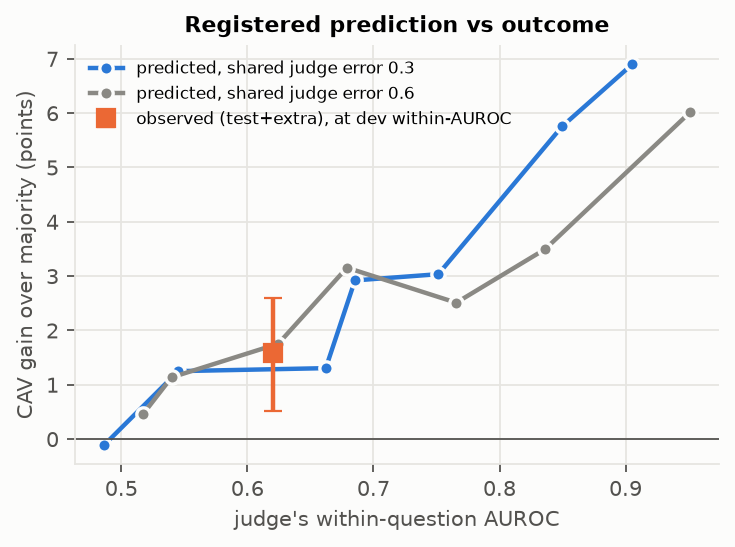
\includegraphics[width=\columnwidth]{figures/prediction_vs_outcome.png}
\caption{CAV gain as a function of the judge's within-question AUROC, predicted before any judging from the real dev
answer structure with simulated judges (lines). The square is the observed pre-registered result on test $\cup$ extra
(95\% CI), placed at the real judge's dev within-question AUROC.}
\label{fig:prediction}
\end{figure}

\paragraph{Cheap verification pays even at small budgets.}
CAV with the direct probability needs only a prefill pass per judged attempt. With $N_1=8$, $m=4$ it reaches
$79.2\%$ at $6.1$ units, $+1.3$ $[+0.8, +1.9]$ over majority vote at the same cost ($+1.3$ $[+0.8, +1.8]$ at matched
tokens). Adaptive-consistency is as good at that budget ($-0.5$ $[-1.2, +0.2]$).

The crossover of \S\ref{sec:scaling} assumed a verdict costs $0.3$ of an attempt. With prefill-only reads, it moves to
smaller budgets, as the cost term predicts.

\paragraph{Argmax is worse than voting; aggregation is not.}
Picking the single attempt with the best verdict probability gives $76.7\%$ at $N=16$, \emph{below} majority vote
($79.8\%$). Summing log-odds over answer groups gives $80.9\%$, as Proposition~2 predicts. CAV gets the aggregation
gain at about half the cost by judging only contested questions.

\paragraph{A learned combination raises AUROC but not picking.}
The exploratory combiner (fitted on dev) raises within-question AUROC on extra to $0.717$ (test $0.666$). It does not
improve CAV accuracy (Table~\ref{tab:selection}). Within-question AUROC averaged over all questions is the wrong
target: the gain has to come from contested questions, where the combiner is still near chance on test.

\begin{table}[t]
\centering\small
\resizebox{\linewidth}{!}{\begin{tabular}{@{}lcccc@{}}
\toprule
& Majority right & Tie & Overturn & Unwinnable \\
\midrule
dev & 0.749 & 0.066 & 0.050 & 0.135 \\
test & 0.723 & 0.062 & 0.042 & 0.173 \\
extra & 0.743 & 0.075 & 0.043 & 0.139 \\
model (test calibration) & 0.717 & 0.080 & 0.030 & 0.172 \\
\bottomrule
\end{tabular}}
\caption{Shares of 4-attempt configurations (random 4-subsets of the 16 attempts). Only ties and overturns can be won by a judge.}
\label{tab:configs}
\end{table}

\begin{table}[t]
\centering\small
\resizebox{\linewidth}{!}{\begin{tabular}{@{}lccc@{}}
\toprule
Rule & Acc. (\%) & Cost & Tokens \\
\midrule
Majority, $N=4$ & 76.0 & 4.00 & 35.7k \\
Majority, $N=8$ & 78.7 & 8.00 & 71.4k \\
Majority, $N=12$ & 79.5 & 12.00 & 107.1k \\
Majority, $N=16$ & 79.8 & 16.00 & 142.8k \\
pass@16 (oracle) & 91.4 & 16.00 & 142.8k \\
Adaptive-consistency, $t=0.8$ & 79.1 & 4.01 & 40.5k \\
Adaptive-consistency, $t=0.9$ & 79.7 & 6.41 & 64.0k \\
Adaptive-consistency, $t=0.99$ & 79.8 & 10.39 & 99.6k \\
Bayes aggregation, $N=4$ & 76.7 & 5.12 & 47.5k \\
Bayes aggregation, $N=16$ & 80.9 & 20.49 & 189.7k \\
Best-of-$N$ argmax, $N=4$ & 75.3 & 5.12 & 47.5k \\
Best-of-$N$ argmax, $N=16$ & 76.7 & 20.49 & 189.7k \\
CAV (chain), $N_1=8$, $m=4$ & 79.0 & 6.70 & 65.2k \\
CAV (direct), $N_1=8$, $m=4$ & 79.2 & 6.09 & 56.1k \\
CAV (combo-cheap), $N_1=8$, $m=4$ & 79.0 & 6.09 & 56.1k \\
CAV (direct), $N_1=12$, $m=4$ & 79.7 & 8.08 & 76.5k \\
CAV (chain), $N_1=12$, $m=8$ & 80.3 & 9.15 & 91.1k \\
CAV (direct), $N_1=16$, $m=4$ & 80.1 & 10.06 & 96.8k \\
CAV (chain), $N_1=16$, $m=8$$^\star$ & 81.0 & 11.31 & 113.9k \\
CAV (combo), $N_1=16$, $m=8$ & 79.6 & 11.31 & 113.9k \\
\bottomrule
\end{tabular}}
\caption{Selection on test $\cup$ extra (800 questions), settings tuned on dev. Cost: attempt $=1$, judge chain $=0.3$, direct read $=0.05$; tokens: decoded tokens per question. $^\star$: pre-registered primary rule.}
\label{tab:selection}
\end{table}


\begin{figure}[t]
\centering
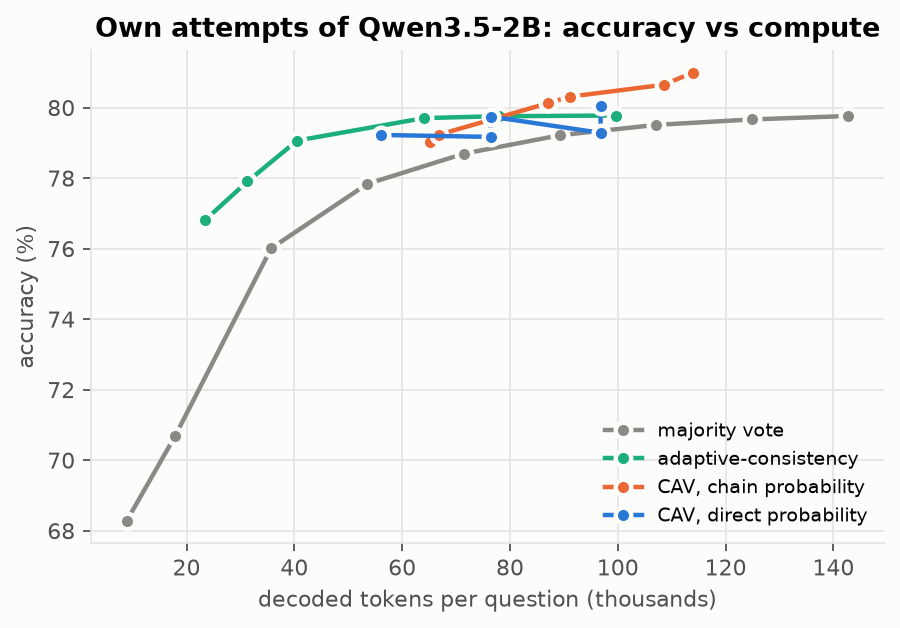
\includegraphics[width=\columnwidth]{figures/real_frontier.png}
\caption{Accuracy against decoded tokens per question on test $\cup$ extra (own attempts of Qwen3.5-2B). Settings
tuned on dev.}
\label{fig:frontier}
\end{figure}

\begin{figure*}[t]
\centering
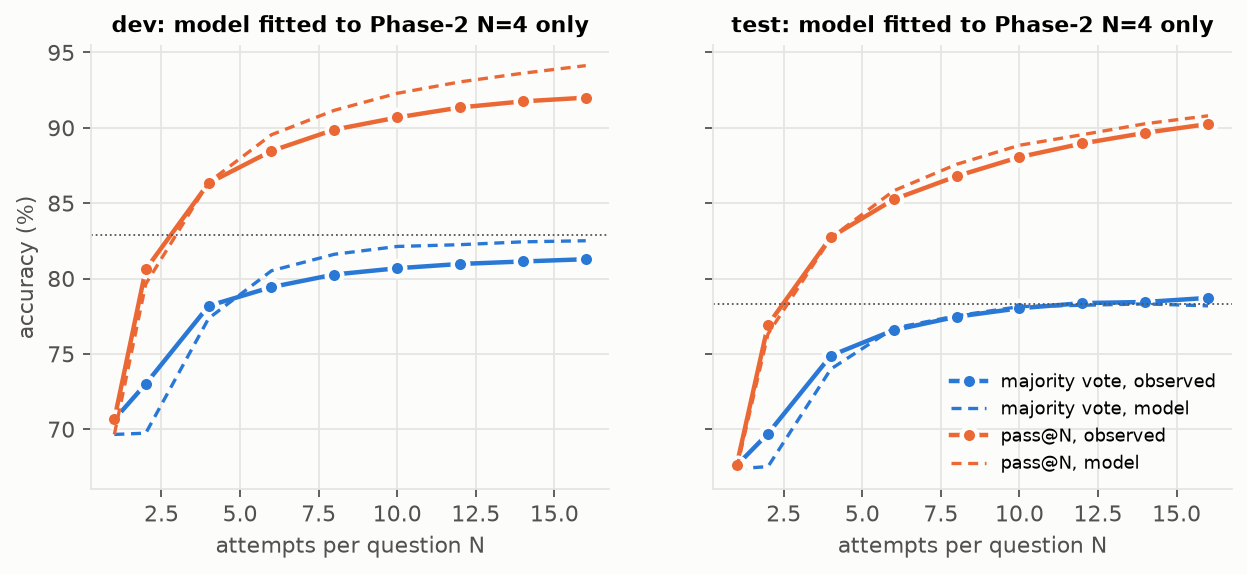
\includegraphics[width=0.8\textwidth]{figures/scaling_observed.png}
\caption{Majority@$N$ and pass@$N$ on own attempts (points) against the model fitted only to Phase-2 4-attempt
aggregates (dashed). Dotted line: the predicted majority limit $P(p_x>\rho(1-p_x))$.}
\label{fig:scaling}
\end{figure*}

\paragraph{Training the judge (future work).}
We also retrained the judge with the Phase-2 recipe in two arms: globally balanced, as in Phase~2, and per-question
balanced (Proposition~3). Verdict reward rose from $40\%$ to $57\%$ and from $48\%$ to $53\%$ respectively; the smaller
rise is consistent with the removed difficulty shortcut. We did not evaluate the trained judges on the selection pools,
so Proposition~3 rests on theory and the learning model of \S\ref{sec:training}.
